\documentclass[12pt,letterpaper]{article}

\usepackage{caption} % for the figure captions
\usepackage[osf]{mathpazo} % a nicer font
% this is a package for the citation formats: found this formulation sorted natbib errors when changing packages
%from http://tex.stackexchange.com/questions/54480/package-natbib-error-bibliography-not-compatible-with-author-year-citations
\usepackage[square,sort,comma,numbers]{natbib} 
\usepackage{amsmath} % package for equations
\usepackage{url} % package for urls
\usepackage{hyperref} % for hyperlinks
\usepackage[a4paper, total={6in, 9in}]{geometry}
\hypersetup{
     colorlinks   = true,
     citecolor    = gray
}
\usepackage{graphicx} % for the figures
\usepackage{pdfpages}

\hypersetup{linkcolor=blue}

\pagenumbering{gobble}

\graphicspath{ }

%Title page
%Itinerary
%Localities
%Kit list
%Contact details
%Where staying: all deets

\begin{document}

%title

{\Huge\textbf{\textit{Ischnacanthus}}\par}
\vspace{3mm}
{\large{Ish-na-can-thus} \par} 
\vspace{5mm}
\textit{Ischnacanthus} is a ``\textbf{spiny shark}'' from the Devonian period - between 420 and 360 million years ago - of Scotland, and had shark-like scales and spines in front of its fins.  
\textit{Ischnacanthus} was a medium-sized acanthodian (about 15-20cm) with \textbf{jaws full of large teeth}, and would have used these to eat smaller acanthodians like \textit{Mesacanthus}.  
We know this because we have the \textbf{coprolites} (fossil poo) of \textit{Ischnacanthus} from the same place as this specimen (Tillywhandland Quarry, Scotland), which are full of smaller scales and spines.\newline

\begin{figure}[h!]
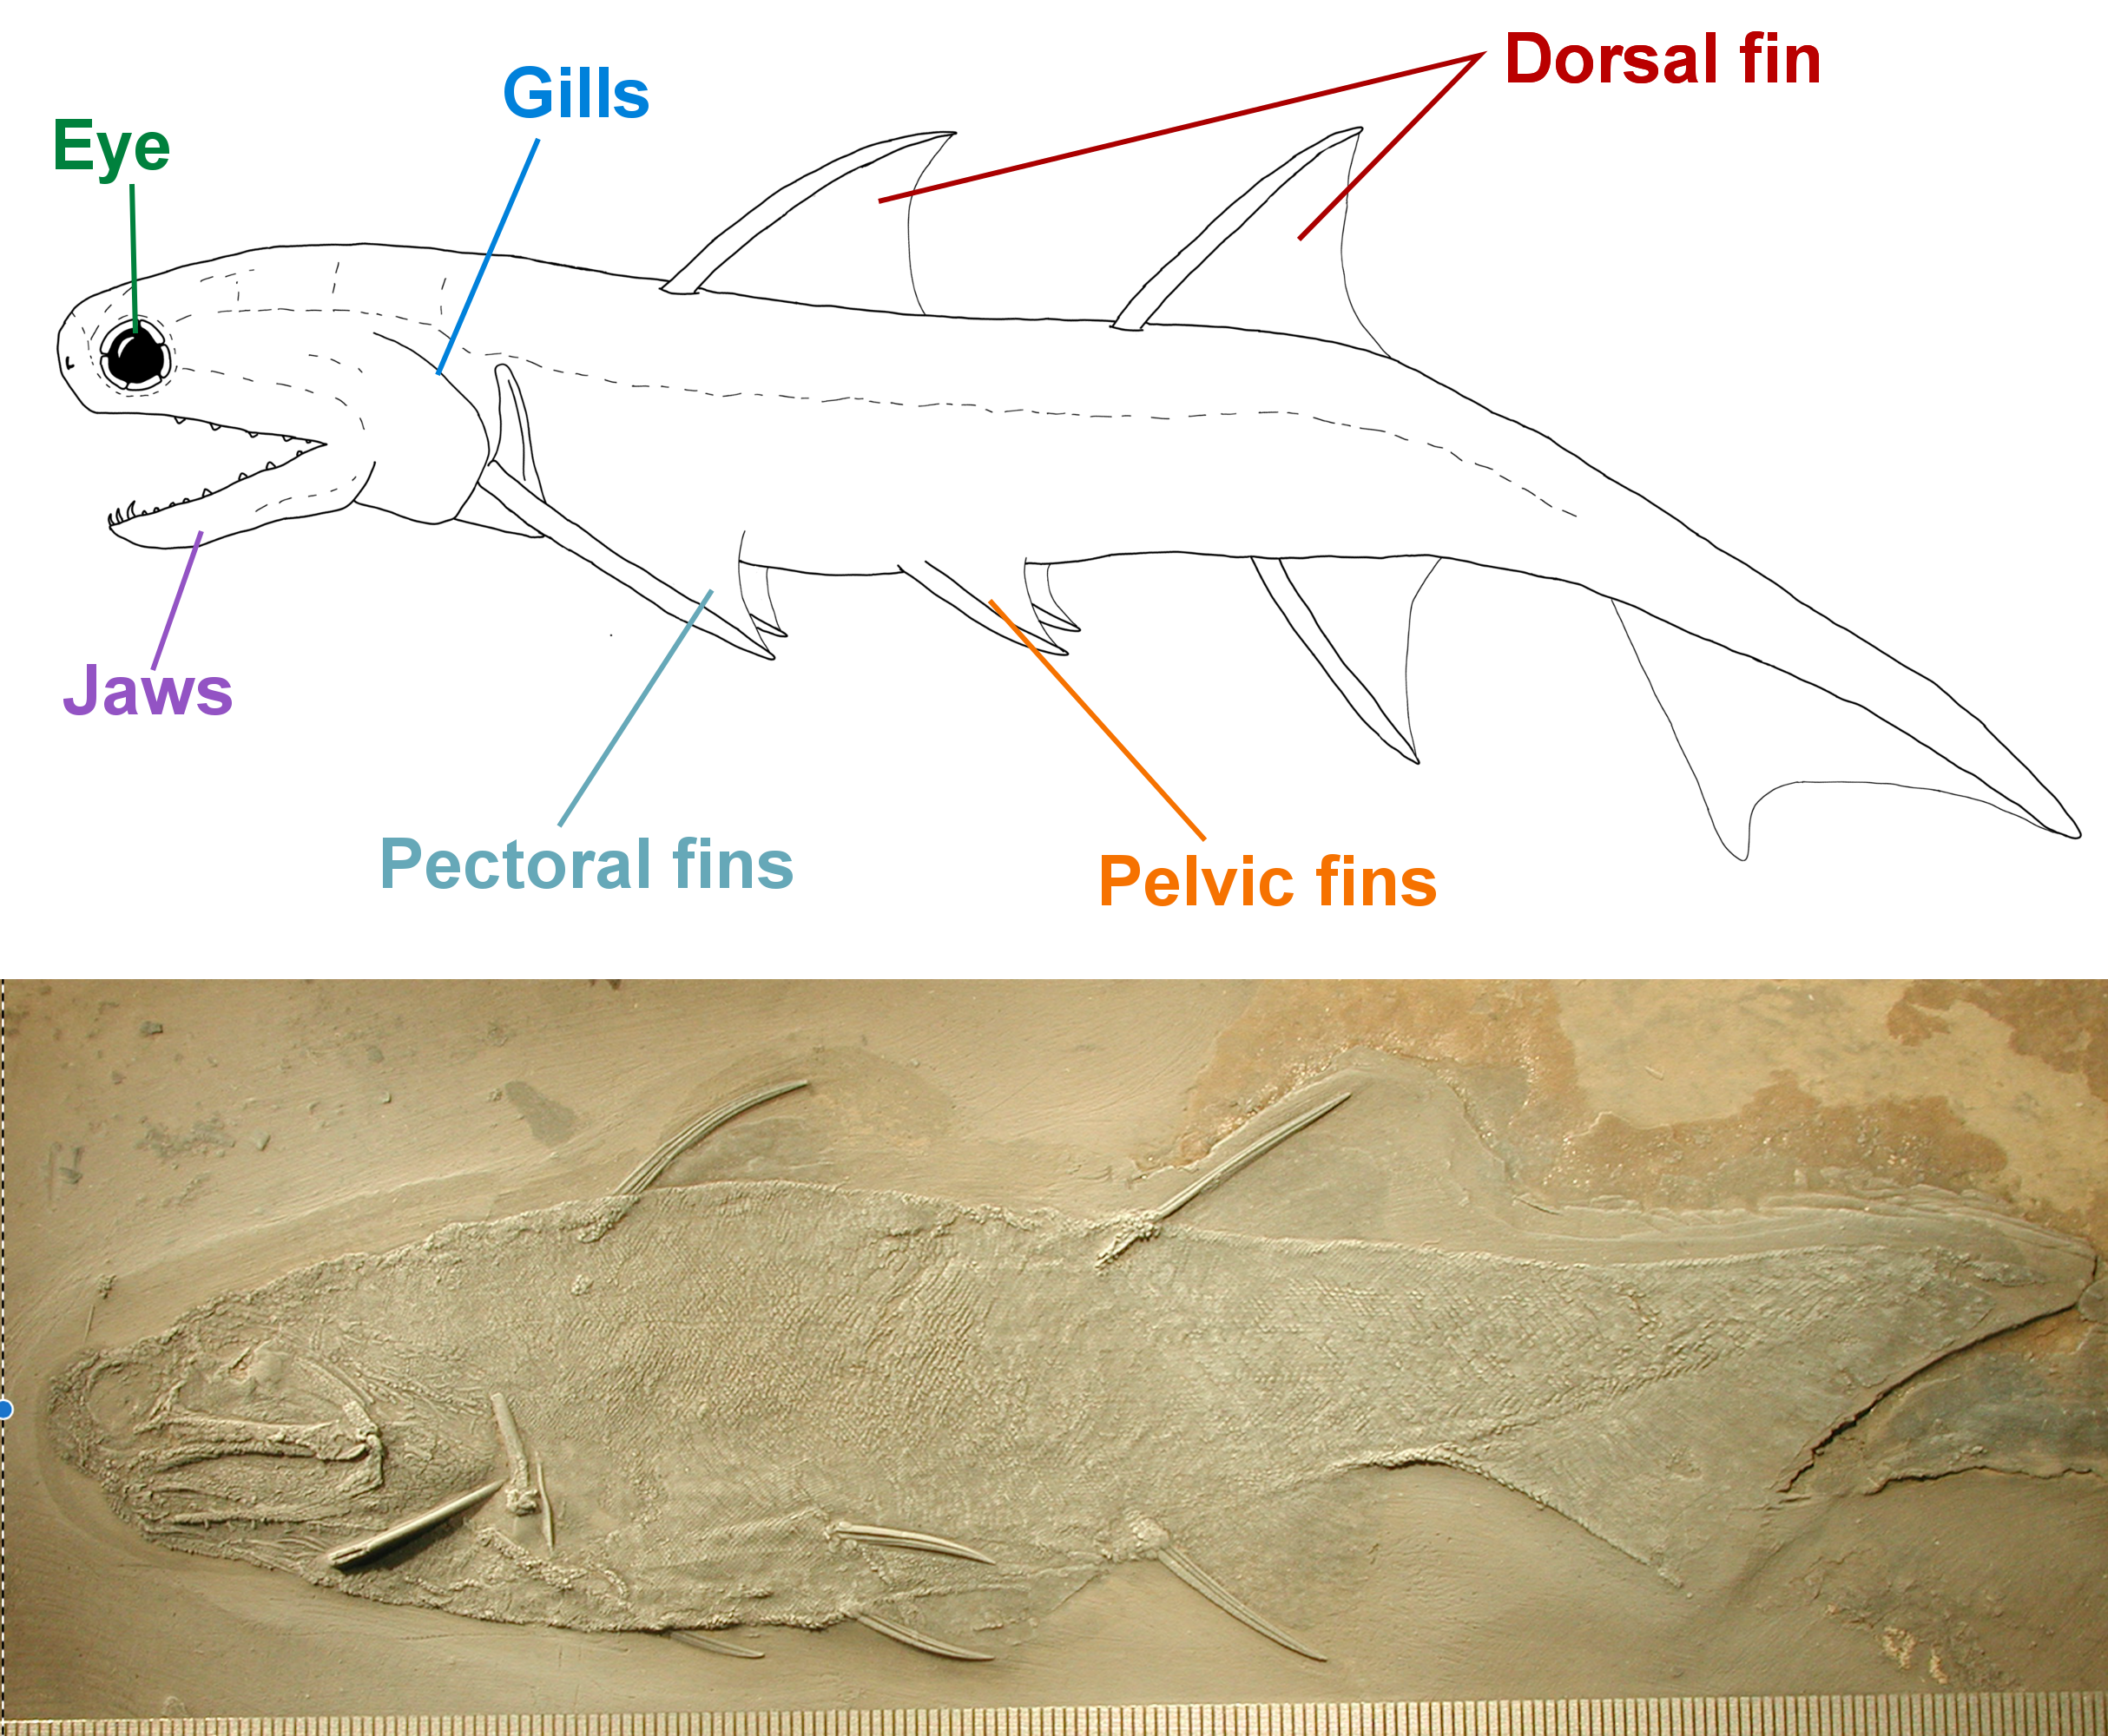
\includegraphics[scale=0.23]{Ischnacanthus}
\centering
\end{figure}

{\large\textbf{\underline{Fossil facts}}\par}

\begin{itemize}
  \item Often the most common fossilised parts of \textit{Ischnacanthus} are its jaws, which are often found apart from the rest of the body.
  \item Unlike living sharks where the teeth fall out and are replaced, in \textit{Ischnacanthus} they are very solidly attached to the jaw.  We know of different kinds of \textit{Ischnacanthus} with teeth that are different shapes.  This tells us that they were using them for feeding on different types of food.
\end{itemize}


\end{document}